\subsection{A* Search with heuristic}
\noindent A* algorithm is one of the popular technique used in path finding and graph traversals. This algorithm completely relies on heuristics for computing the future cost of a problem. This algorithm is equivalent to the uniform cost search with modified edge cost. This heuristics is chosen according to the case where the algorithm is implemented, thus emphasizing the importance of domain knowledge. This algorithm is consistent if the modified cost is greater than zero.

\begin{figure}[H]
	\centering
	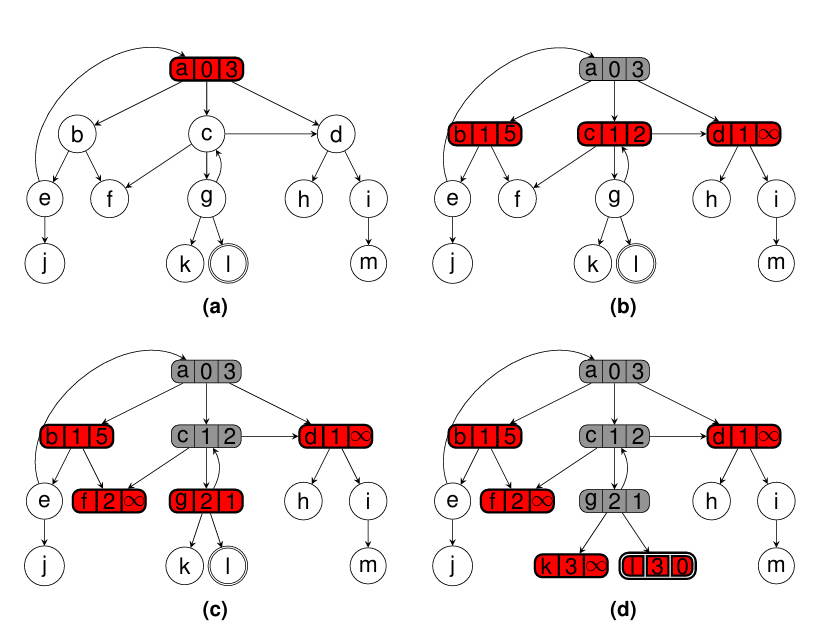
\includegraphics[width=0.8\textwidth]{./imgs/astar.png}
	\caption{A* Algorithm}
\end{figure}

\subsubsection{Pseudocode}
\begin{algorithm}[H]
	\caption{A* Search (\textit{start, goal, heuristic})}
	\label{alg:astar}
	\begin{algorithmic}[1]
	\State priority queue $\gets$ [(start, cost = 0, estimated total cost = heuristic(start))]
	\While {priority queue is not empty}
		\State (node, cost) $\gets$ dequeue(priority queue)
		\If {node = goal}
			\State return path
		\EndIf
		\ForAll {neighbor in valid moves}
			\State new cost $\gets$ cost + move cost
			\State estimated total cost $\gets$ new cost + heuristic(neighbor)
			\If {neighbor not visited or new cost $<$ previous cost}
				\State mark neighbor as visited
				\State enqueue(priority queue, (neighbor, new cost, estimated total cost))
			\EndIf
		\EndFor
	\EndWhile
	\State return failure
	\end{algorithmic}
\end{algorithm}

\subsubsection{Implementation}

\subsubsection{Time and Space Complexity}